\scanpage{111}

\[
\Sigma_J=\mathbb{P}(V(J))\simeq\check{\mathbb{P}}(V(J))
\]
\diagram{\begin{tikzcd}[ampersand replacement=\&]
\cdot \arrow[r,dash] \& V(J) \arrow[r] \& \mathcal{O}^J \arrow[r,"\text{sum}"',/tikz/arrows={-|}] \& \mathcal{O} \arrow[r] \& 0
\end{tikzcd}}

\deleted{Sequence}
\diagram{\begin{tikzcd}[ampersand replacement=\&]
0 \arrow[r] \& F \arrow[r] \& V(J)_\Sigma \arrow[r] \& \mathcal{O}_\Sigma(1) \arrow[r,dash] \& 0
\end{tikzcd}}

\[
F(1)\simeq\mathcal{O}(\omega)
\qquad
(\mathcal{O}\ \text{twisted by }\underline{\omega}=\underline{\omega}(J)\deleted{\unsure{)}},\ \text{i.e. }\det V(J))
\]
\[
\mathcal{O}(1)\simeq\check{F}(\omega)
\qquad
\left(\text{by }F\wedge\underline{\mathcal{O}}_\Sigma(1)
\mathrel{\mathop{\simeq\!\longrightarrow}\limits_{\text{exterior product}}}
\det V(J)_\Sigma\simeq\mathcal{O}_\Sigma(\omega){}_{\deleted{\Sigma}}\right)
\]
\margin{watch the signs!}
\margin{$+$}

\margin{%
$F\times V(J)\longrightarrow\underline{\mathcal{O}}$

Pairing given (\deleted{fixing} a fixed cyclic order \deleted{taking} $(i,j,k)$), by
$x\wedge y\wedge e_i=x\wedge y\wedge e_j=x\wedge y\wedge e_k$
where $x\in F$, $y\in V(J)$ modulo $F$
i.e. given by the \inserted{\unsure{3|2}} minors -
of the matrix of $(x,y)$.
}

\[
\underline{\Omega}^1_\Sigma\deleted{\unsure{0}}\simeq F(-1)\simeq\mathcal{O}(\unsure{-2})(\underline{\omega})
\]
\[
\underline{\check{\Omega}}^1_\Sigma\simeq\mathcal{O}(2)(\underline{\omega})
\qquad\text{tangent bundle : }\Sigma
\]

\margin{$\deleted{\unsure{\varphi_{ij}+\varphi_{jk}+\varphi_{ki}=0}}$}

Points 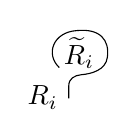
\begin{tikzpicture}[baseline=(base.base),x=1cm,y=1cm]
\node[inner sep=0pt] (base) at (-0.46,-0.57) {$R_i$};
\node[inner sep=0pt] (r) at (0,0) {$\inserted{\widetilde{R}_i}$};
\draw (-0.25,-0.19)
 .. controls (-0.43,-0.02) and (-0.33,0.26) .. (-0.03,0.28)
 .. controls (0.27,0.31) and (0.39,0.16) .. (0.36,-0.06)
 .. controls (0.34,-0.22) and (0.16,-0.27) .. (0.03,-0.28)
 .. controls (-0.06,-0.29) and (-0.13,-0.33) .. (-0.13,-0.42)
 -- (-0.13,-0.58);
\end{tikzpicture} $(i\in J)$ (``holes'') of $\Sigma$ and $P\Sigma$

\[
\begin{gathered}
R_i\subset\unsure{\mathbb{V}|V}(J)\\
\Vert\\
\mathcal{O}_{\unsure{k|\Sigma}}(e_k-e_j)\\
\simeq\mathcal{O}(\underline{\omega})
\end{gathered}
\qquad\mathcal{O}(1)_{R_i}\simeq\mathcal{O}
\]
by associating to $e_k-e_j$ the orientation $(i,j,k)$

\margin{%
$\widetilde{R}_i$ point over $R_i$
image of $e_i-e_j=\varphi_{ji}$
$(\equiv e_i-e_k)$ in $V(J)/R_i$
}

\deleted{Points the $\widetilde{R}_i$ of $P\Sigma_J=\check{V}^{*}(\mathcal{O}_\Sigma(1))$ the element $1$ over $R_i$.}

\[
\Gamma(\Sigma_{\deleted{J}},\mathcal{O}_\Sigma(1))\simeq V(J)
\]
\deleted{$e_j-e_k$ section $\omega_{j,k}$}
\[
\varphi_{jk}=e_k-e_j\in\Gamma(\Sigma,\underline{\mathcal{O}}_\Sigma(1))
\]
vanishing at $R_i$
\[
\varphi_{kj}=-\varphi_{jk}\qquad\varphi_{jk}(R_i)=0
\]
\margin{$\varphi_{ij}+\varphi_{jk}+\varphi_{ki}=0$.}
\[
\boxed{\varphi_{jk}(R_k)=\widetilde{R}_k\quad\varphi_{jk}(R_j)=-\widetilde{R}_j}
\]
\margin{watch the signs!}

Points $Q_i$ $(i\in J)$, $Q_i^\omega{}_{\deleted{\unsure{\omega}}}$ $(i\in J,\omega\in\underline{\omega})$

\[
\begin{gathered}
Q_i\subset\unsure{\mathbb{V}|V}(\underline{J})\\
\Vert\\
\mathcal{O}(-2e_i+\deleted{\unsure{0}}(e_j+e_k))
\end{gathered}
\qquad\mathcal{O}(1)_{Q_i}\simeq\mathcal{O}(\underline{\omega})
\]

\margin{%
the two distinguished points of $\mathcal{O}(\omega)_{Q_i}^{*}$,
indexed by $\underline{\omega}$ are denoted $Q_i$, $Q'_i$,
or $Q_{i,\omega}$ $((i,\omega)\in J\times\underline{\omega}$
}

\inserted{\figure{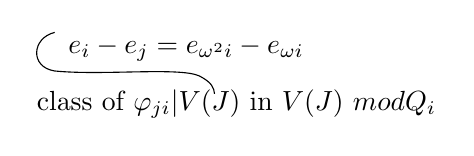
\begin{tikzpicture}[x=1cm,y=1cm]
\node[anchor=west] (eq) at (0,0.7) {$e_i-e_j=\unsure{e_{\omega^2i}-e_{\omega i}}$};
\node[anchor=west] (cl) at (-0.4,0) {class of $\deleted{\unsure{\varphi_{ji}|V(J)}}$ in $V(J)\ \text{mod }Q_i$};
\draw (-0.05,0.91) .. controls (-0.34,0.84) and (-0.37,0.47) .. (-0.05,0.42)
 .. controls (0.55,0.36) and (1.52,0.47) .. (1.78,0.36)
 .. controls (1.96,0.27) and (1.97,0.2) .. (1.98,0.13);
\end{tikzpicture}}}

\deleted{by $\varphi_{\omega i,\omega^2i}(Q_i)=$}

\[
\boxed{Q_i^\omega{}_{\deleted{\unsure{\omega}}}=
\underset{\deleted{\unsure{\varphi_{i,\omega^2i}}}}
{\overset{\inserted{\varphi_{\omega i,i}}}
{\deleted{\unsure{\varphi_{i,\omega i}}}}}(Q_i)}
\]

\margin{NB $\boxed{Q_i^{\omega^{-1}}{}_{\deleted{\unsure{\omega^{-1}}}}=-Q_i^\omega{}_{\deleted{\unsure{\omega}}}}$

$\varphi_{\omega i,\omega^2i}(Q_i)=2Q_i^\omega{}_{\deleted{\unsure{\omega}}}$}

thus
\[
\widetilde{Q}_i=\varphi_{jk}(Q_i),\quad
\widetilde{Q}'_i=-\varphi_{jk}(Q_i)=\varphi_{kj}(Q_i)
\]

Points $P_\omega$ $(\omega\in\underline{\omega}_J)$,
$P_i^\omega{}_{\deleted{\unsure{\omega}}}$ $(i\in J,\omega\in\omega)$.
Let $\zeta$ be a \deleted{$\unsure{\zeta}$} primitive cube root of $1$ (we shall take \deleted{$\unsure{\zeta}$}
\[
\zeta=\exp 2i\pi/3
\]
then

\mspage{110}
